\chapter{Модель интеллектуальной системы принятия решений для регистрации и анализа проблемных ситуаций в ИТ-инфраструктуре предприятия} \label{chapt3}

В данной главе рассмотрены модели, которые были изучены и использованы при создании системы принятия решений для регистрации и анализа проблемных ситуаций в ИТ-инфраструктуре предприятия. Отметим, что работа над системой велась с 2011 года, за истекшее время было создано три рабочих версии прототипа системы, реализующих различные модели мышления. \par
Созданными и испытанными моделями, использованными при создании системы принятия решений для регистрации и анализа проблемных ситуаций в ИТ-инфраструктуре предприятия, являются:
 \begin{itemize}
	\item модель Menta 0.1, построенная с использованием деревьев принятия решений;
	\item модель Menta 0.3, построенная с использованием генетических алгоритмов \cite{ArtificialIntelligence} ;
	\item модель TU 1.0, основанная на модели мышления Марвина Мински  \cite{EmotionMachine}.
\end{itemize}

Модель, построенная на базе нейронных сетей (поддерживающая обучение), была отброшена на предварительной стадии оценки, так как она предъявляет большие требования к производительности (скорости работы и требуемых ресурсов)\cite{NEURAL}, что в свою очередь порождает высокую стоимость. Далее каждая модель будет рассмотрена подробно.

%====================

%====================
\section{Построение модели Menta 0.1 с использованием деревьев принятия решений} \label{sect3_1}
Данная модель была одной из первых, которые были апробированы. Она основана на деревьях принятия решений \cite{DTREE}, которые широко используются в вопросно-ответных системах \cite{DC1, DC2, DC3}. При построении модели использованы компоненты, реализующие обработку запросов на естественном языке, поиск решения, применение найденного решения, хранение в базе знаний.\par
Система ориентирована на выполнение таких простых команд, как, например, «Добавить поле в форму». Основные функции модели представлены следующими потоками: получение и формализация запроса; поиск решения при помощи деревьев принятия решений; изменение приложения согласно запросу; генерация и компиляция приложения. Рассмотрим подробнее, как устроена система. Начнем с того, как в системе представлены данные.

\subsection{База знаний на основе OWL}
Для представления данных в системе была использована база знаний, построенная на основе OWL-файла (см. \cite{OWL}). С помощью редактора Protege \cite{Protege} в базу вводились начальные данные о целевом приложении (приложении, которое будет модифицироваться системой согласно запросам пользователей) в виде семантической сети. В качестве такого приложения была создана система, которая вела учет заказов пользователя на покупку того или иного товара в интернет-магазине. \par

 На рисунке \ref{img:order-owl} представлен один из программных классов (согласно терминологии ООП \cite{Meyer}) этой системы~--- Order~--- в формате OWL. Этот класс отвечает за обработку заказов. Слева отображены супер классы (классы-предки), к которым он привязан. Например, класс BLL относится к бизнес-логике приложения, Module~--- отдельный модуль в рамках системы. Справа представлены свойства класса, а их описания приведены в таблице \ref{OrderPropertyDescription}. С помощью предикатов определяется поведение свойства: создать файл, создать новое поле. В таблице \ref{Predicates} представлено описание иерархии предикатов. На рисунке \ref{img:CreateCustomer} представлен класс CreateCustomer в OWL, в который входит описание всех необходимых свойств для генерации файла исходного кода на языке Java.

\begin{figure} [h] 
  \center
  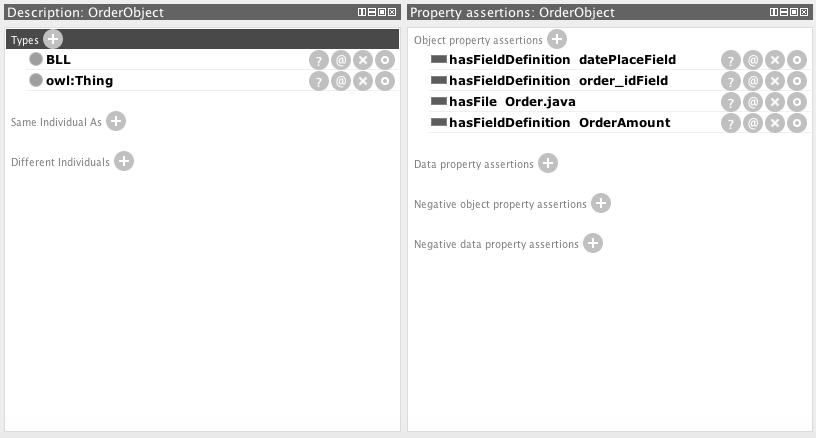
\includegraphics [scale=0.7] {OrderOWL}
  \caption{Представление класса Order в OWL. Визуализация Protege} 
  \label{img:order-owl}  
\end{figure}


\begin{table} [htbp]
  \centering
  \parbox{15cm}{\caption{Описание свойств класса Order в OWL}\label{OrderPropertyDescription}}
%  \begin{center}
  \begin{tabular}{| p{3cm} | p{4cm} | p{8cm} |}
  \hline
 \textbf{Свойство} & \textbf{Предикат} & \textbf{Описание} \\
  \hline
    OrderAmount	& hasFieldDefinition & Поле: сумма заказа \\
  \hline
orderidField	& hasFieldDefinition & Поле: идентификатор заказа \\
  \hline
Order.java	& hasFile & Идентификатор имени файла для генерации \\
  \hline
datePlaceField	& hasFieldDefinition & Поле: время размещения заказа \\
  \hline
    \end{tabular}
%  \end{center}
\end{table}

\begin{table} [htbp]
  \centering
  \parbox{15cm}{\caption{Описание иерархии предикатов}\label{Predicates}}
%  \begin{center}
  \begin{tabular}{| p{5cm} | p{10cm} |}
  \hline
  
\textbf{Предикат} & \textbf{Описание} \\
  
    \hline
 hasFieldDefinition & Предикат, обозначающий свойство класса \\
  \hline
 hasMethodDefinition & Предикат, обозначающий функцию \\
  \hline
classDefinition & Обозначение класса \\
  \hline
database & Обозначение базы данных\\
  \hline
    \end{tabular}
%  \end{center}
\end{table}

\begin{figure} [h] 
  \center
  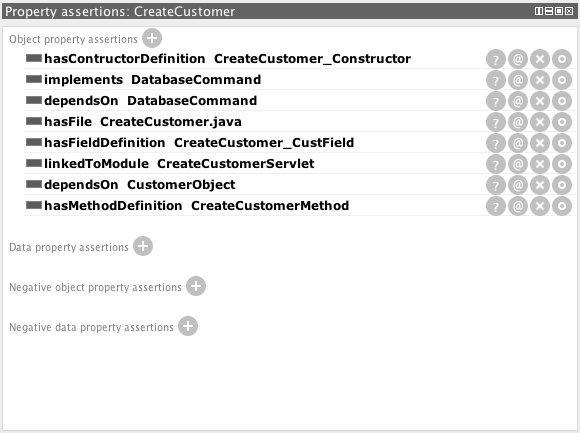
\includegraphics [scale=0.7] {CreateCustomer}
  \caption{Представление класса CreateCustiner в OWL. Визуализация Protege} 
  \label{img:CreateCustomer}  
\end{figure}
\clearpage
\subsection{Основные компоненты модели}
Основными компонентами модели являются: Request parser (Stanford parser); Генерация Action (Action Generator); Исполнение Action (Action Applier); Генерация приложения (Application Generator). \par
\emph{Request parser} формализует запрос на естественном языке. \emph{Action Generator} генерирует объект класса Action (который содержит описание требуемых над моделью приложения действий) из результатов работы, основываясь на Деревьях принятия решений \cite{DCFOREST} и базе данных. Основной задачей данного модуля является генерация имени, действия и поля. Модуль \emph{Action Applier} отыскивает объект в модели по данным от Action Generator и производит действие, кроме того, используя предикат dependOn, он производит модификацию всех зависимых классов. \par
 В модели поддерживается два типа Action: RemoveFieldAction (удаление поля), AddFieldAction (добавление поля). После завершения работы производится генерация целевого приложения на языке Java при помощи OWL-модели в модуле \emph{Application Generator}. На рисунке \ref{img:MentaUseCase} представлена UML-диаграмма последовательности для основного рабочего потока приложения: пользователь вводит в систему запрос "Add new field to Customer (Добавить новое поле в класс Customer)"; модуль StanfordParser вычленяет из запроса связи типа dobj (связь объекта и действия); модуль ActionGenerator создает на основе связей объект, описывающий список действий (далее~--- действие) над моделью, для получения требуемого результата; модуль ActionApplier, используя действие, изменяет модель приложения; модуль ApplicationGenerator применяет изменения к приложению. В результате у класса Customer (данный класс содержит набор свойств, необходимых для описания клиента магазина) появляется новое поле "New". \par
\begin{figure} [h] 
  \center
  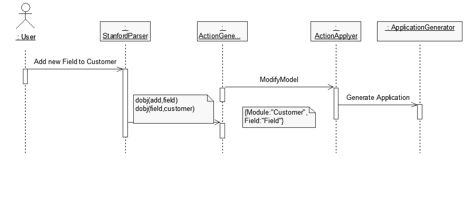
\includegraphics [scale=1.2] {MentaUseCase}
  \caption{UML-диаграмма последовательности для основного потока в модели Menta 0.1} 
  \label{img:MentaUseCase}  
\end{figure}
После проведения экспериментов было выявлено, что приложение не может использовать ранее найденные решения, абстрагируя их. Например, система знает, как произвести операцию добавления поля, но вот аналогичную операцию~--- добавить метод~--- сделать не может. Поиск решения также потребовал специального обучения: система не могла путем перебора информации в своей базе знаний найти решение.  В системе также не было возможности обучения. \par
После применения этой системы была предпринята попытка найти более универсальное решение. Результатом стало построение модели Menta 0.3, описанной ниже.

%===============================
\section{Модель Menta 0.3, построенная с использованием генетических алгоритмов} \label{chapt2}
В данную модель по сравнению с предыдущей были добавлены модуль логики для оценки решения и модуль генетических алгоритмов для генерации решения. Отметим, что генетические алгоритмы часто применяются в биологически инспирированных системах \cite{G1}, \cite{G3}. Кроме того, есть примеры их использования в системах поддержки принятия решений, однако эффективность таких систем не подтверждена \cite{G2}. В рамках модели Menta 0.3 были отработаны следующие основные компоненты будущей итоговой модели: критерии приемки (Acceptance Criteria); How-To~--- для хранения решений проанализированных проблем; формат данных OWL; использование логических вычислений для проверки решения. Система Menta 0.3 содержала внутри себя модель целевого приложения (как и Menta 0.1) и список решений тех или иных проблем (How-To). При помощи генетического алгоритма модель строила решение (How-To), проверяла его при помощи логического движка NARS \cite{NARS} на соответствие входным критериям приемки. С точки зрения генетических алгоритмов это~--- функция отбора особей из поколения \cite{GFITNESS}. 

\subsection{Основные компоненты модели}
Модель состоит из компонентов, представленных в Таблице \ref{ModulesMenta03}.

\begin{longtable}{|p{5cm}|p{11cm}|}
 \caption[Компонетны модели Menta 0.3]{Компонетны модели Menta 0.3}\label{ModulesMenta03} \\ 
 \hline
 
 \multicolumn{1}{|c|}{\textbf{Компонент}} & \multicolumn{1}{c|}{\textbf{Описание}}  \\ \hline 
\endfirsthead
\multicolumn{2}{c}%
{{\bfseries \tablename\ \thetable{} -- продолжение}} \\
\hline \multicolumn{1}{|c|}{\textbf{Компонент}} &
\multicolumn{1}{c|}{\textbf{Описание}}  \\ \hline 
\endhead


\endfoot

\hline \hline
\endlastfoot
 MentaController & Веб-служба \cite{WebService}, которая предоставляет интерфейс для общения с пользователем и остальными системами \\
  \hline
 SolutionGenerator & Модуль отвечает за генерацию решения. На вход он получает Acceptance Criteria. Основой является генетический алгоритм. Для него был выбран framework ecj \cite{ECJ}. Из всех возможных классов в базе знаний, отсеянных по классификатору, составляются паросочетания. К каждому паросочетанию применяется логическое суждение на основе AcceptanceCriteria (за это отвечает модуль ReasonerAdapter). В итоге паросочетание получает оченку в виде пары Frequency, Confidence (частота, вероятность). 
Таким образом находится наилучшее паросочетание. Если его показатель 1,1, то решение принимается, иначе отбрасывается (на данный момент установлен жесткий показатель).
SolutionGenerator включает в себя SolutionChecker, который включает в себя ReasonerAdapter.
 \\
  \hline
SolutionChecker & Проверка решения. Принимает на вход выбранные How-To, AcceptanceCriteria. Комбинирует их и передает ReasonerAdapter. \\
  \hline
ReasonerAdapter & Транслирует  How-To в термины NARS. NARS~--- non-axiomatic reasoning system \cite{NARS} (система логических суждений, разработанная профессором Пеем Вонгом). Принцип действия NARS~--- это всевозможная комбинация фактов. Каждый факт имеет свои частоту и вероятность. Их сочетанием получается композиция данных фактов.\\
  \hline
  Translator & Транслирует объекты базы знаний (знания) в отчеты. Последние бывают следующих типов: Solution Report; UML Report; Patch. В данной версии используется первый тип отчета. Он содержит описание на выбранном языке программирования решения, найденного системой.\\
  \hline
  Applicator & Данный модуль применяет решение к модели приложения, содержащейся в базе знаний. Также данная модель включает FileApplicator, который генерирует решение в виде файлов на выбранном языке программирования. \\
  \hline
  KBServer & База знаний приложения. Используется сервер non-SQL БД HypergraphDB. \\
  \hline
%  \end{center}
\end{longtable}
В предыдущей модели в качестве хранения данных использовался файл, что было неудобно в случае, если приложение работает параллельно с несколькими запросами. В системе Menta 0.3 был использован специальный сервер баз данных, речь о котором пойдет далее.

\subsection{База знаний на основе графов}
При реализации базы знаний (здесь и далее~--- KBServer) был создан промежуточный модуль доступа к данным (здесь и далее~--- DAO, Data Access Object), данный подход широко используется в проектировании программного обеспечения \cite{THREELAYERARCH}. Это позволяет максимально отделить реализацию KBServer от конкретного хранилища. \par 

\textbf{EntityManagerFactory}. Данный класс является входной точкой и создает объект, с помощью которого приложение осуществляет работу с базой знаний. Класс автоматически выбирает необходимые настройки для объекта. \par

\textbf{EntityManager}. Это основной класс для загрузки и хранения объектов из базы данных.\par

\textbf{Configuration}. Этот класс хранит такие параметры настройки базы данных, как физическое положение БД и максимальное количество подключений. \par 
\textbf{EntityTransaction}. Данный класс используется для управления транзакциями при доступе к объектам базы данных. \par
При выборе физического хранилища данных было проанализировано несколько хранилищ OWL-данных: OWLIM, SESAME и HG. Результаты их сравнения представлены в таблице \ref{DatabaseEngineComparison}.
\begin{longtable}{|p{6cm}|p{3cm}|p{3cm}|p{3cm}|}
 \caption[Сравнение скорости доступа к данным баз знаний]{Сравнение скорости доступа к данным баз знаний}\label{DatabaseEngineComparison} \\ 
 \hline
 
 \multicolumn{1}{|c|}{\textbf{}} & \multicolumn{1}{c|}{\textbf{Sesame}} & \multicolumn{1}{c|}{\textbf{OWLIM}} & \multicolumn{1}{c|}{\textbf{HG}} \\ \hline 
\endfirsthead
\multicolumn{2}{c}%
{{\bfseries \tablename\ \thetable{} -- продолжение}} \\
\hline \multicolumn{1}{|c|}{\textbf{}} & \multicolumn{1}{c|}{\textbf{Sesame}} & \multicolumn{1}{c|}{\textbf{OWLIM}} & \multicolumn{1}{c|}{\textbf{HG}} \\ \hline 
\endhead

\endfoot

\hline \hline
\endlastfoot
 \textbf{Единицы измерения} & \textbf{мс.} & \textbf{мс.} & \textbf{мс.} \\
  \hline
 предварительно скомпилированные запросы & 26 253 & 3 012 & 6 813 \\
  \hline
 без кеша & 30 545 & 1 122 & 9 045 \\
  \hline
 с кешем & 24 258 & 962 & 985 \\
%  \end{center}
\end{longtable}

Несмотря на то, что OWLIM дает лучшие результаты, был выбран HGDB, который предоставляет более широкие возможности доступа к данным, такие, например, как поддержка алгоритмов работы с графами.

%========================================
%========================================

\section{Модель TU 1.0, основанная на модели мышления Марвина Мински}
Следующим этапом разработки стала модель, построенная с применением теории Марвина Мински. Эта модель сохранила следующие основные концептуальные элементы предыдущих моделей и показала свою состоятельность на контрольных примерах: Acceptance Criteria; Обучение; Поиск и применение решения; Отсутствие обработки естественного языка. Данная модель является более универсальной и представляет собой верхнеуровневую архитектуру обработки запроса (мышления), где компонентами являются лучшие части предыдущих систем.
\subsection{Особенности модели мышления}
В 2006 году Марвин Мински опубликовал свою книгу "The emotion machine" \cite{EmotionMachine}, в которой предложил свой взгляд на систему мышления и памяти человека. В основу его теории легла парадигма триплета \triplet\ (далее \tripletshort), k-line (линия, которая связывает приобретенные знания, например, огонь~--- горячо) для сопоставления знаний. На рисунке \ref{img:csw} представлено схематичное изображение \tripletshort. \par
\begin{figure} [h] 
  \center
  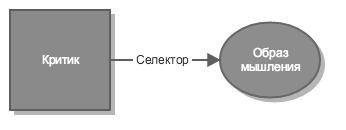
\includegraphics [scale=1.0] {csw}
  \caption{\triplet} 
  \label{img:csw}  
\end{figure}

\textbf{Критик} представляет собой определенный переключатель: внешние обстоятельства, события или иное воздействие. Например, «включился свет, и зрачки сузились», «обожглись и одернули руку». Критик активируется только тогда, когда для этого достаточно обстоятельств. Одновременно может активироваться несколько критиков. Например, человек решает сложную задачу, идет активация множества критиков: выполнить расчет, уточнить технические детали. Кроме того, параллельно может активироваться критик, сообщающий о необходимости отдыха.\par
\textbf{Селектор} занимается выбором определенных ресурсов, одним из которых является Образ мышления. \par
\textbf{Образ мышления}~--- это способ решения проблемы. Образ мышления может быть сложным и способен активировать других критиков. Например, размышляя над проблемой, специалист понимает, что нужно произвести полный перебор всех возможных комбинаций параметров, чтобы получить нужный результат, и тут он решает поискать готовое решение: а может кто-то уже сделал такой перебор, и можно будет использовать его результаты. Здесь «поиск готового решения» является критиком внутри образа мышления «поиск решения». \par

На рисунке \ref{img:csw_ex} представлена расширенная модель работы \tripletshort. Критик активирует Селектор, который активирует Образ мышления (овал). Последний в свою очередь может активировать нового Критика или же совершить определенные действия. Например, зажегся зеленый свет светофора, значит, можно переходить дорогу. Под ресурсами здесь понимается набор знаний из базы знаний: Критики, Селекторы, Образы мышления, готовые решения.
 \par
Если активировалось много Критиков, то проблему нужно уточнить, так как степень неопределенности слишком высока. Если проблема очень похожа на уже проанализированную, то можно действовать и судить по аналогии.
\begin{figure} [h] 
  \center
  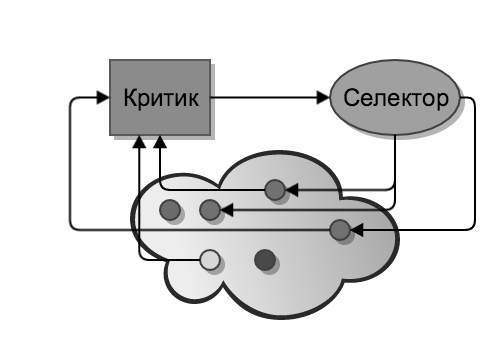
\includegraphics [scale=0.8] {csw_ex}
  \caption{\tripletshort\  в разрезе ресурсов} 
  \label{img:csw_ex}  
\end{figure}


\subsection{Основные компоненты модели}
\textbf{Уровни мышления}\par
Концепция уровней мышления представляет собой модель степени ментальной активности человека. Никто из людей не может похвастаться скоростью гепарда, гибкостью кошки или силой медведя. На наш взгляд, все это компенсируется возможностью изобретения образов мышления. Например, чтобы быть быстрыми, люди изобрели различные механизмы (самолеты, машины и др.). Чтобы быть сильными, они изобрели оружие. \par
 Все изобретения являются результатом взаимодействия человека с окружающим миром. Именно данное взаимодействие заставляет людей изобретать что-то новое, создавать шедевры литературы и летать в космос. По ходу своего развития разум человека проходит путь от врожденных инстинктов до возможности создания фундаментальных трудов, таких как  «Теории всего» \cite{Hawking}. В этом ему помогает возможность гибкого мышления: изобретение различных подходов к решению проблемы. Далее мы рассмотрим концепцию уровней мышления, следуя Марвину Мински \cite{EmotionMachine}. \par
Начнем с описания уровней мышления, которое представлено в таблице \ref{ThinkingLevelDescription}. Деление на данные уровни носит условный характер. Например, уровни 5 и 6 можно объединить, но, по словам Марвина Мински, принцип бритвы Оккама, который успешно применяется в физике, не должен также легко и однозначно применяться в психологии и теории мышления. \par




\begin{longtable}{|p{5cm}|p{11cm}|}
 \caption[Описание уровней мышления, предложенных Марвином Мински]{Описание уровней мышления, предложенных Марвином Мински}\label{ThinkingLevelDescription} \\ 
 \hline
 
 \multicolumn{1}{|c|}{\textbf{Уровень}} & \multicolumn{1}{c|}{\textbf{Описание}} \\ \hline 
\endfirsthead
\multicolumn{2}{c}%
{{\bfseries \tablename\ \thetable{} -- продолжение}} \\
\hline \multicolumn{1}{|c|}{\textbf{Уровень}} & \multicolumn{1}{c|}{\textbf{Описание}} \\ \hline 
\endhead

\endfoot

\hline \hline
\endlastfoot
Инстинктивный уровень & Происходят инстинктивные реакции (врожденные). Например, коленный рефлекс. Общую формулу для этого уровня можно выразить как «если ..., то сделать так». \\
  \hline

Уровень обученных реакций & Используются накопленные знания, то есть те знания, которым человек обучается в течение жизни. Например, переходить дорогу на зеленый свет. Общую формулу для этого уровня можно описать как «если ..., то сделать так». \\
  \hline

Уровень рассуждений & Мышление с использованием рассуждений. Например, если перебежать дорогу на зеленый свет, то можно успеть вовремя. На данном уровне сравниваются последствия нескольких решений и выбирается оптимальное. Общую формулу для этого уровня можно выразить как «если ..., то сделать так, тогда будет так». \\
  \hline

Рефлексивный уровень & Рассуждения с учетом анализа прошлых событий. Например, «в прошлый раз я побежал на моргающий зеленый и чуть не попал под машину». \\

  \hline
  Саморефлексивный уровень & Построение определенной модели, с помощью которой идет оценка своих поступков. Например, «мое решение не пойти на это собрание было неверным, так как я упустил столько возможностей, я был легкомысленным». \\
  \hline
  Самосознательный уровень & Оценка своих поступков с точки зрения высших идеалов и оценок окружающих. Например, «а что подумают мои друзья? А как бы поступил мой герой?» \\
  \hline

\end{longtable}


На рисунке \ref{img:thinkinglevels} представлено схематичное изображение уровней мышления, названных выше. 1--3 уровни составляют личность человека. 2--5 представляют ЭГО человека (Человеческое Я)~--- осознание человека в общении с окружающими. 3--6 представляют собой сверх ЭГО человека (сверх Я)~--- его моральные установки.
\begin{figure} [h] 
  \center
  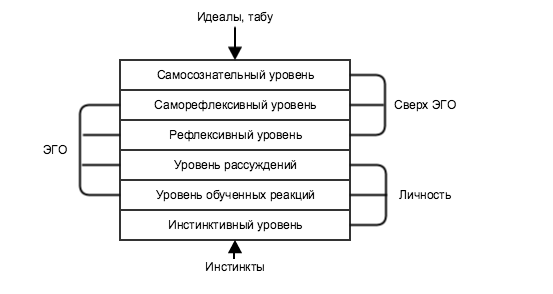
\includegraphics [scale=1.0] {thinkinglevels}
  \caption{Иллюстрация концепции Уровней мышления} 
  \label{img:thinkinglevels}  
\end{figure}


\textbf{Концепция k-line}. Эта концепция была первый раз упомянута Марвином Мински в 1987 году в журнале Cognitive Science. В книге \cite{SocietyOfMind} Марвин Мински раскрывает концепцию k-line. Полностью концепция описана позже в книге \cite{EmotionMachine}. 
K-line представляет собой связь между двумя событиями, объединяющими их в знание, например, объединение Образа мышления, найденного решения и активированной проблемы. 

На рисунке \ref{img:k_line} показана k-line, которая объединяет образы мышления, решения и других Критиков. Данная концепция позволяет «запоминать» удачные решения. 
\clearpage
\begin{figure} [h] 
  \center
  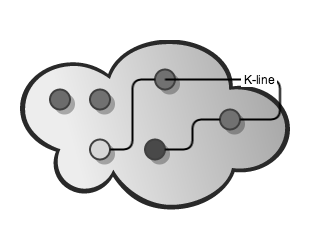
\includegraphics [scale=1.0] {k_line}
  \caption{Иллюстрация концепции k-line} 
  \label{img:k_line}  
\end{figure}
\section{Выводы по главе 2}
Модель Menta 0.1 имеет следующие недостатки: отсутствие устойчивости к грамматическим и содержательным ошибкам входной информации. Например, входной файл не имел отношения к программной системе, модель которой была в базе знаний в формате OWL; система поиска решения работала только в рамках модели одной программы; отсутствовала функция обучения. \par
В данный момент существует новый подход, который использует леса деревьев принятия решений \cite{DCFOREST}, он в рамках данной модели не рассматривался. Модель Menta 0.3 имеет следующие недостатки: отсутствие обучения; отсутствие обработки естественного языка; модуль HyperGraphDB оказался непригодным для промышленного использования; NARS в виду своих особенностей оказался непригодным для промышленного применения на значительном объеме фактов (>20), так как содержал в себе комбинаторный взрыв\footnote{Комбинаторный взрыв~--- термин, используемый для описания эффекта резкого («взрывного») роста временной сложности (до бесконечности) алгоритма при увеличении размера входных данных задачи.}. Например, при 10 фактах количество сочетаний будет равно 45 на первом уровне, далее алгоритм NARS будет сравнивать результаты этих сочетаний. Кроме того, после апробации оказалось, что критерии приемки практически описывают необходимое решение, что является недопустимым. Данный подход был описан в статье \cite{SoftwareAutomation}. \par

Для программной экспертной системы очень важно обладать способностью мыслить и рассуждать, например, очень важно для системы уметь проводить аналогии между уже известными разрешениями проблем и вновь появившимися. Множество запросов типично и отличается лишь параметрами. Например, пожалуйста, установите Office, Antivirus \etc\ \par
Также для экспертной системы важно уметь абстрагировать специализированные рецепты решения. К примеру, система научилась решать инцидент "Please install Firefox"\ («Пожалуйста, установите Firefox»). Абстрагировав данный инцидент до степени "Please install browser"\  («Пожалуйста, установите браузер»), система сможет теми же способами попробовать разрешить новую проблему.\par
После рассмотрения нескольких моделей была выбрана модель мышления Марвина Мински, так как она может быть адаптирована на области разрешения проблемных ситуаций, возникающих в процессе эксплуатации ИТ-инфраструктуры предприятия. На основе подхода Мински была построена модель системы, которая поддерживает основные функции: обучение, понимание инцидента, поиск решения, применение решения. 

\clearpage

